\documentclass[review]{elsarticle}
\usepackage[T1]{fontenc}
\usepackage[utf8]{inputenc}
\usepackage{lineno}
\usepackage[demo]{graphicx}
\usepackage{amsmath}
\usepackage{xcolor}
\usepackage{amssymb}
\usepackage{amsthm}
\usepackage{upquote}
\usepackage{fullpage}
\usepackage{listings}
\usepackage{hyperref} 
% \definecolor{mygreen}{rgb}{0,0.6,0}
% \definecolor{mygray}{rgb}{0.5,0.5,0.5}
% \definecolor{mymauve}{rgb}{0.58,0,0.82}
\everymath{\displaystyle}  % math equations
% \abovedisplayskip=12pt
% \belowdisplayskip=12pt
% \abovedisplayshortskip=0pt
% \belowdisplayshortskip=7p % math equations
\definecolor{codegreen}{rgb}{0,0.6,0}
\definecolor{codegray}{rgb}{0.5,0.5,0.5}
\definecolor{codepurple}{rgb}{0.58,0,0.82}
\definecolor{backcolour}{rgb}{0.95,0.95,0.92}
% \lstset{ %
% language=Python,                % choose the language of the code
% basicstyle=\footnotesize,       % the size of the fonts that are used for the code
% numbers=left,
% formfeed=newpage,                    % where to put the line-numbers
% numberstyle=\footnotesize,      % the size of the fonts that are used for the line-numbers
% stepnumber=1,                   % the step between two line-numbers. If it is 1 each line will be numbered
% numbersep=5pt,                  % how far the line-numbers are from the code
% backgroundcolor=\color{white},  % choose the background color. You must add \usepackage{color}
% showspaces=false,               % show spaces adding particular underscores
% showstringspaces=false,         % underline spaces within strings
% showtabs=false,                 % show tabs within strings adding particular underscores
% frame=single,           % adds a frame around the code
% tabsize=2,          % sets default tabsize to 2 spaces
% captionpos=b,           % sets the caption-position to bottom
% breaklines=true,        % sets automatic line breaking
% breakatwhitespace=false,    % sets if automatic breaks should only happen at whitespace
% escapeinside={\%*}{*)}          % if you want to add a comment within your code
% }
\lstset{
  language=Python,                 % the language of the code
  %backgroundcolor=\color{white},   % choose the background color; you must add \usepackage{color} or \usepackage{xcolor}; should come as last argument
  basicstyle=\footnotesize,        % the size of the fonts that are used for the code
  breakatwhitespace=false,         % sets if automatic breaks should only happen at whitespace
  breaklines=true,                 % sets automatic line breaking
  captionpos=b,                    % sets the caption-position to bottom
  %commentstyle=\color{mygreen},    % comment style
  %deletekeywords={...},            % if you want to delete keywords from the given language
  %escapeinside={\%*}{*)},          % if you want to add LaTeX within your code
  extendedchars=true,              % lets you use non-ASCII characters; for 8-bits encodings only, does not work with UTF-8
  frame=single,                    % adds a frame around the code
  keepspaces=true,                 % keeps spaces in text, useful for keeping indentation of code (possibly needs columns=flexible)
 % keywordstyle=\color{blue},       % keyword style
  morekeywords={print, append, DropoutLayer, rectify, layers, InputLayer, init},    % if you want to add more keywords to the set
 % identifierstyle=\color{purple},
 backgroundcolor=\color{backcolour},   
 commentstyle=\color{codegreen},
 keywordstyle=\color{magenta},
 numberstyle=\tiny\color{codegray},
 stringstyle=\color{codepurple},
  numbers=left,                    % where to put the line-numbers; possible values are (none, left, right)
  numbersep=5pt,                   % how far the line-numbers are from the code
  %numberstyle=\tiny\color{mygray}, % the style that is used for the line-numbers
  rulecolor=\color{black},         % if not set, the frame-color may be changed on line-breaks within not-black text (e.g. comments (green here))
  showspaces=false,                % show spaces everywhere adding particular underscores; it overrides 'showstringspaces'
  showstringspaces=false,          % underline spaces within strings only
  showtabs=false,                  % show tabs within strings adding particular underscores
  stepnumber=2,                    % the step between two line-numbers. If it's 1, each line will be numbered
  %stringstyle=\color{mymauve},     % string literal style
  tabsize=2,                       % sets default tabsize to 2 spaces
  title=\lstname                   % show the filename 
}
\modulolinenumbers[5]
%\usepackage[square]{natbib} 
%\usepackage[a4paper]{geometry}
%\usepackage{url, hyperref} 
%\usepackage[svgnames]{xcolor}
%\usepackage{xcolor}
%\usepackage[utf8]{inputenc}
%\usepackage{graphicx}
%\usepackage{upquote}
%elsarticle-template.tex 

\journal{CMPS-185}

%%%%%%%%%%%%%%%%%%%%%%%
%% Elsevier bibliography styles
%%%%%%%%%%%%%%%%%%%%%%%
%% To change the style, put a % in front of the second line of the current style and
%% remove the % from the second line of the style you would like to use.
%%%%%%%%%%%%%%%%%%%%%%%

%% Numbered
%\bibliographystyle{model1-num-names}

%% Numbered without titles
%\bibliographystyle{model1a-num-names}

%% Harvard
%\bibliographystyle{model2-names.bst}\biboptions{authoryear}

%% Vancouver numbered
%\usepackage{numcompress}\bibliographystyle{model3-num-names}

%% Vancouver name/year
%\usepackage{numcompress}\bibliographystyle{model4-names}\biboptions{authoryear}

%% APA style
%\bibliographystyle{model5-names}\biboptions{authoryear}

%% AMA style
\usepackage{numcompress}\bibliographystyle{model6-num-names}

%% `Elsevier LaTeX' style
%\bibliographystyle{elsarticle-num}
%\bibliographystyle{IEEEtran}
%%%%%%%%%%%%%%%%%%%%%%%

\begin{document}
\begin{frontmatter}
\title{Convolutional Neural Networks for Pattern Matching in Poker-Type Games}

% \tnotetext[mytitlenote]{Fully documented templates are available in the elsarticle package on \href{http://www.ctan.org/tex-archive/macros/latex/contrib/elsarticle}{CTAN}.}

%% Group authors per affiliation:
% \author{Elsevier\fnref{myfootnote}}
% \address{Radarweg 29, Amsterdam}
% \fntext[myfootnote]{Since 1880.}
\author{James M. Vrionis }
\address{Santa Cruz, California}


%% or include affiliations in footnotes:
% \author[mymainaddress,mysecondaryaddress]{Elsevier Inc}
% \ead[url]{www.elsevier.com}

% \author[mysecondaryaddress]{Global Customer Service\corref{mycorrespondingauthor}}
% \cortext[mycorrespondingauthor]{Corresponding author}
% \ead{support@elsevier.com}

% \address[mymainaddress]{1600 John F Kennedy Boulevard, Philadelphia}
% \address[mysecondaryaddress]{360 Park Avenue South, New York}

%--------------------------------------------------------------------------
% (3) An abstract

\begin{abstract} 
The imperfect information game poker is a stochastic family of card 
matches defined by a card-dealing and betting. Ranks assigned to 
singleton cards and combinations of those cards will Outcomes of each 
game can are dependent on the different combinations of cards relative 
to rank. The supposition in which the majority of poker games can be 
solved as pattern matching problems has inspired the creation of a 
strong user-agent based on unified poker representation. An iterative 
self-play training method that incorporates prior game actions to 
continually develop and optimize its proficiency in poker. This 
user-agent named {\ttfamily"}Poker-CNN{\ttfamily"} learns to predict 
the best strategy directly from the previous cards and bets without 
being reliant on sophisticated domain knowledge. This approach is 
applied to three different poker variations: single player video poker, 
two-player Limit Texas Hold'em and Two-player 2-7 triple draw. Poker-CNN 
can quickly learn patterns in these three different types of poker 
games while gaining experience from itself improvements 
ultimately reaching human expert skill level from heuristic players.\\ 
{\ttfamily"}The contributions of this paper include: (1) a novel 
representation for poker games, extend-able to different poker 
variations, (2) a convolutional Neural Network (CNN) based learning 
model that can effectively learn the patterns in three different games, 
and (3) a self-trained system that significantly beats the heuristic-based 
program on which it is trained, and our system is competitive against 
human expert players.{\ttfamily"}
\end{abstract}

%--------------------------------------------------------------------------

% \begin{keyword}
% \texttt{elsarticle.cls}\sep \LaTeX\sep Elsevier \sep template
% \MSC[2010] 00-01\sep  99-00
% \end{keyword}

\end{frontmatter}

\linenumbers

% (4) Well-defined sections with headers and some content in each of them
% (6) The overall structure of the term paper (sections with titles)
\section{Preliminaries}

\begin{itemize}
    \item Definitions of important concepts
    \item Notation and Terminology
    \item Results from other articles that will be used in the sequel.
\end{itemize}

\section{Background}

%------------------------------------------------------------------------
Stochastic games have been a desirable field of research because skill
can be determined objectively. This may be true for many games like
checkers or chess whereas the many different poker variations can be 
thought of something way more complex. 

The weights of the convolutional neural network have a replicated 
structure which applies the same weights to every subrectangle of 
the image producing the total inputs to the next layer. The weights 
of a convolutional neural network are also called the convolutional 
kernel, $K$, and its size, $n$, is the size of the subrectangles it 
considers. \\

\begin{figure}[convectVSFullyConnect]
    \centering
    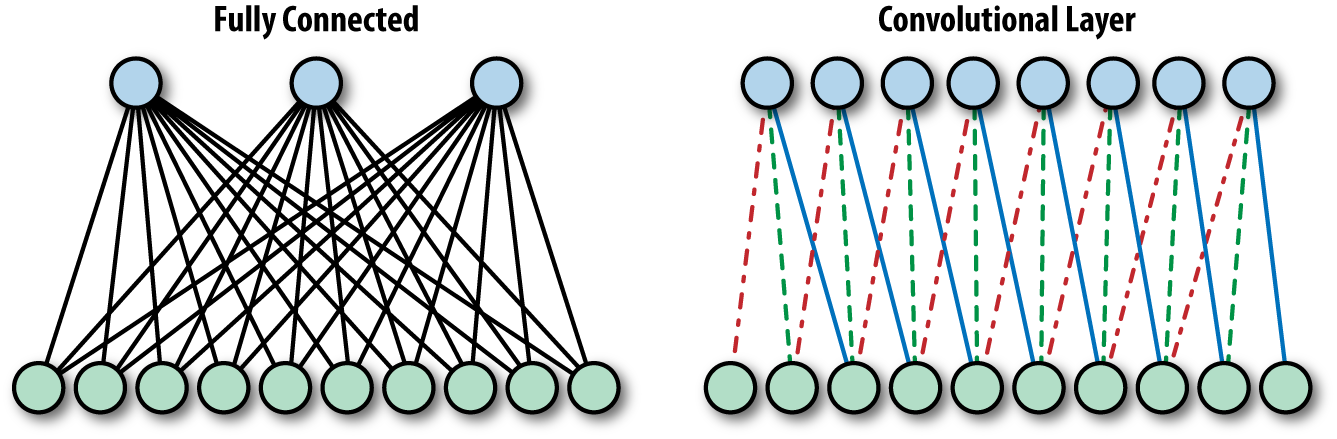
\includegraphics[width=\textwidth,height=6cm,keepaspectratio=true]{convectVSFullyConnect}
    \caption{
        Fully Connected Neural Net vs CNN ~\cite{ConvecFCN}
    }
    \label{fig:FCN vs. CNN}
\end{figure}

Convolutional neural networks form a subclass of feedforward 
neural networks that have special weight constraints. CNNs facilitate 
learning  at a much higher rate of efficiency given fewer examples when 
two-dimensional translation invariance is evident. 
It's important to realize a fully connected feedforward neural network 
has a very large number of parameters when compared to a CNN of the same size. 
Small number of weights make parameter estimation a necessity to determine 
if a good can be found quickly. ~\cite{ISutskeve2008} \\


\begin{equation*}
y_{x,y} = \left(1 + exp \left(  -\sum_{u=-(n-1)/2}^{(n-1)/2}
            \sum_{v=-(n-1)/2}^{(n-1)/2} x_{x+u,y+v} K_{u,v} \right) \right)
\end{equation*}\\

where $y$ is the activity of a hidden unit at position $(x,y)$, and $x$ 
are the input units.~\cite{ISutskeve2008} \\
%------------------------------------------------------------------------

%------------------------------------------------------------------------
The objective of Poker-CNN is to use CNN and a ranking system applied to three 
tensor-based frameworks. This will develop a general learning model designed to 
teach itself how to play and in time, dominate professional human players at 
many different types of poker games. \\
%------------------------------------------------------------------------


%------------------------------------------------------------------------
\section{Related Work}
Counterfactual Regret Minimization is used as a solution to heads-up
No Limit Texas Hold'em. Given some game state, 
this method will examine every possible outcome to eventually reach 
an equilibrium solution using different search strategies. Domain 
knowledge and massive amounts of data are necessary for CFRs to develop 
an effective user-agent. It's important to mention on of the most 
successful implementations of a CFR based Neural Network. 
DeepStack ~\cite{Moravcik2017}, a CFR based solution to Texas 
Hold'em, does carry the title of the first 
computer program to defeat professional poker players at heads-up 
No-limit Texas Hold'em (NLTH), an imperfect information 
game with over $10^{160}$ games states. ~\cite{MJohanson2013} \\

The process uses recursive reasoning of CFR to handle information 
asymmetry. Prior to play DeepStack does not compute and store a complete 
strategy. Instead, situations are considered in real time, examining 
each particular situation accordingly.  
This is accomplished using a standard feed-forward network 
containing seven fully connected hidden layers each containing 500 nodes 
and parametric rectified linear units (28) for the output. DeepStack 
takes pot-size and players ranges as a function of the public cards as 
inputs and will output vectors of counterfactual values for each player 
and hand as fractions of the pot size. This is the first computer program 
to beat professional poker players in No-Limit Texas 
Hold'em, it's approach dramatically reduces worst-case
exportability when compared to the abstraction paradigm of Poker-CNN. \\
%------------------------------------------------------------------------

%------------------------------------------------------------------------
An important distinction that must presented is the difference between 
perfect and imperfect information games. Games like chess and backgammon 
can be defined as perfect information games because both players know 
the state of the game at all times. When any type of action is taken 
or performed the true nature of this action is known to all other 
participants involved whereas imperfect information can are 
simultaneous in nature. Each new game state is can be regarded as 
the starting state of a new game. By comparison, strategies for a 
perfect information game is much easier to implement, especially 
when defined relative to each decision point.\\
Value-based reinforcement learning such as TD- and Q-learning are
powerless towards imperfect counterparts. With that in mind a gradient 
search performed on the parameter spaces simultaneously shift probability
distributions in a more successful outcome. This special case of the 
lagging anchor algorithm promotes much better results.
~\cite{ Dfredrik2001} \\

%------------------------------------------------------------------------

%------------------------------------------------------------------------
\section{Games of Poker}

\subsection*{Video Poker}
\paragraph{Video poker (VP) is a single-player game of draw poker, 
easily found in many casinos. The house randomly deals five cards 
for a $1\$$ dollar fee and shortly after one can either keep their 
current cards or trade-in some number of cards (1-5) from one to 
five for a new set of card(s). The objective of VP is 
simple: match the best possible hand of five cards Given 32 
possible choices, based on the players{\ttfamily\char'15} final 5 
cards where payout is calculated by a table of matches.} \\
~\cite{YakovenkoCRF15}\\

\subsection*{Limit Poker}
\paragraph{(heads-up limit) Texas Hold'em (LTH): Heads-Up limit Texas Hold'em, is two 
player card game lasting four rounds with no more than four bets per round.  
Both players have a fixed amount of money known as \textit{stack size} at 
the start of each game. An ante is required to start every game and is 
considered the first round of betting where one player is responsible for 
\textbf{small blind} whilst the other must pay the \textbf{big blind} 
(a max of three additional bets during this round). Private and public 
cards are dealt and if the players make it through 3 more rounds a showdown
will take place which is where both players end up showing each other 
their hands where there is only one winner.}
~\cite{MJohanson2013}.\\

\subsection*{2-7 Triple Draw}
Just like (heads-up limit) Texas Hold'em, 2-7 Triple Draw Poker is a 
multi-round game capable of many players. This game is like a mixture of 
the previous two games, which means this variation of poker would be 
the most difficult to develop a model for that would be competitive 
against professional human players. Just like LTH this game has multiple
rounds of betting but in this game you can also choose to trash some number
of your cards or keep them. Another difference this game exhibits is low 
card is high, in other words a low card straight would be the best hand.
~\cite{YakovenkoCRF15}. \\

%------------------------------------------------------------------------


% a general solution using CNNs for different types 
% of poker. Using competitive gain(s) to loss(es) ratio. Self-taught 
% (Simple heuristic players) Ultimately, Poker-CNN must be competitive
% against professional human players

% \paragraph{Installation} If the document class \emph{elsarticle} is not available on your computer, you can download and install the system package \emph{texlive-publishers} (Linux) or install the \LaTeX\ package \emph{elsarticle} using the package manager of your \TeX\ installation, which is typically \TeX\ Live or Mik\TeX.

% \paragraph{Usage} Once the package is properly installed, you can use the document class \emph{elsarticle} to create a manuscript. Please make sure that your manuscript follows the guidelines in the Guide for Authors of the relevant journal. It is not necessary to typeset your manuscript in exactly the same way as an article, unless you are submitting to a camera-ready copy (CRC) journal.




%----------------------------------------------------------------------------------------
% The Body of the article contains a detailed presentation of the results of the article.
% The content of the Body should, for the most part, represent original work not found elsewhere 
%(unless it is a survey article).
% The content of the Body is what justifies writing the article.  
% All other parts of the article are to support the Body.
% The Body typically consists of several sections.
% Each section has a separate heading suggesting its content.
% Each section should focus on one particular theme, which should be fully developed and thoroughly explored.
% The sections should have roughly comparable length.
% Avoid having a very long section and a very short section.
% A section may have several subsections.
%----------------------------------------------------------------------------------------
% \section{Games of Poker}

% \subsection{Video Poker}
% \paragraph{}
% One player and one round.
% Insert a dollar and receive five arbitrary picked cards.
% A player is allowed to trade-in up to five cards for new cards. 
% Final Hand determines payout.


% \subsection{Limit Poker}
% \paragraph{Heads$-$up} Texas Hold'em game played in the ACPC is a
%  two player games with four rounds and at most four bets per round. In the 
%  first round, the players' small blind and big blind (an ante required to 
%  start the game), counts as a bet, and at most three additional bets are allowed. 
%  The public and private cards are dealt out as normal for Texas Hold'em games. ~\citeMJohanson2013}.

% \subsection{2-7 Triple Draw}
% \paragraph{}

% Five cards, multiplayer game.
% Player can either draw nothing or up to three new cards betting in-between.
% Notice TDP has draws like VP and betting like TH. 
% It is called $2-7$ because lowest hand wins.

%----------------------------------------------------------------------------------------
% \subsection{No Limit Texas Hold {\textquotesingle}em}
\section{Poker Relational Model: URP}
\paragraph{Helper function to turn a poker hand (array of cards) into 2D array.
if pad\_to\_fit then pass along to card input creator, to create $14x14$ array instead of $4x13$
NOTE: $17x17$ padding!
NOTE: Double\_row $= T$ expands to $8x13$ by repeating suit row. Full order: CDHS CHDS.
Idea is that any pair can be learned with a single convolution. (Any two suit rows together.)}

%----------------------------------------------------------------------------------------
\subsection{Tensor Representation}
\begin{lstlisting}[language=Python, caption=Unified Representation for Poker Games]
HAND_TO_MATRIX_PAD_SIZE = 17
DOUBLE_ROW_HAND_MATRIX = True # False # True # False # Set true for 8x13 matrix, with redundancy. 
remap_suit = {CLUB:CLUB, HEART:DIAMOND, DIAMOND:HEART, SPADE:SPADE}
def hand_to_matrix(poker_hand, pad_to_fit=False, pad_size=HAND_TO_MATRIX_PAD_SIZE, double_row=DOUBLE_ROW_HAND_MATRIX):
    # initialize empty 4x13 matrix
    # Unless pad to fit... in which case pad to 17x17
    if pad_to_fit:
        matrix = np.array([[0 for x in range(pad_size)] for x in range(pad_size)], np.int32)
    else:
        matrix = np.array([[0 for x in range(len(ranksArray))] for x in range(len(suitsArray))], np.int32)
    if pad_to_fit:
        if pad_size == 17:
            # add 5 empty rows to start, and 5 empty rows to finish
            suit_offset = 6
            # add empty column to start 
            value_offset = 2
        elif pad_size == 15:
            suit_offset = 5
            value_offset = 1
        if double_row:
            suit_offset -= 2
    else:
        suit_offset = 0
        value_offset = 0

    for card in poker_hand:
        #print card
        #print ([suits_to_matrix[card.suit]], [card.value])
        matrix[suits_to_matrix[card.suit] + suit_offset][card.value + value_offset] = 1

    # If double row, now copy rows
    if double_row:
        suit_offset += 4
        for card in poker_hand:
            matrix[suits_to_matrix[remap_suit[card.suit]] + suit_offset][card.value + value_offset] = 1
        
    return matrix
\end{lstlisting}
~\cite{moscow25} \\
%----------------------------------------------------------------------------------------

%----------------------------------------------------------------------------------------
\section{Poker Games}



% Card suits and ranks in 2D.
% CNN model Poker-CNN
% two convolutional layers, one maxpooling layer, two more convolutional layers, 
% one more maxpooling layer ,one dense layer, dropout layer, 
% filter size is 5 $\times$ 5

%----------------------------------------------------------------------------------------
\subsection*{Big Filters}

CNN model Poker-CNN, two convolutional layers, one maxpooling layer, 
two more convolutional layers, one more maxpooling layer ,one dense layer, 
dropout layer, filter size is 5 $\times$ 5 \\

Model with 5x5 filter on the bottom for Better visualization while 
tracking all the layers creating and this will return a full stack.

\begin{lstlisting}[language=Python, caption=Big Filter Encoding]
def build_fat_model(input_width, input_height, output_dim,
                    batch_size=BATCH_SIZE, input_var = None):
    print('building fat model, layer by layer...')
    num_input_cards = FULL_INPUT_LENGTH
    layers = []
    l_in = lasagne.layers.InputLayer(
        shape=(batch_size, num_input_cards, input_height, input_width),
        input_var = input_var,
        )
    layers.append(l_in)
    print('input layer shape %d x %d x %d x %d' 
                % (batch_size, num_input_cards, input_height, input_width))
    l_conv1 = lasagne.layers.Conv2DLayer(
        l_in,
        num_filters=NUM_FAT_FILTERS,
        filter_size=(5,5),
        nonlinearity=lasagne.nonlinearities.rectify,
        W=lasagne.init.GlorotUniform(),
        )
    layers.append(l_conv1)

   
    l_conv2_2 = lasagne.layers.Conv2DLayer(
        l_conv2,
        num_filters=NUM_FAT_FILTERS*2,
        filter_size=(3,3),
        nonlinearity=lasagne.nonlinearities.rectify,
        W=lasagne.init.GlorotUniform(),
        )
    layers.append(l_conv2_2)
    print('convolution layer l_conv2_2. Shape %s' % str(l_conv2_2.output_shape))

    # Skip second max-pool.
    l_hidden1 = lasagne.layers.DenseLayer(
        l_conv2_2, #l_pool2,
        num_units=NUM_HIDDEN_UNITS,
        nonlinearity=lasagne.nonlinearities.rectify,
        W=lasagne.init.GlorotUniform(),
        )
    layers.append(l_hidden1)

    print('hidden layer l_hidden1. Shape %s' % str(l_hidden1.output_shape))

    l_hidden1_dropout = lasagne.layers.DropoutLayer(l_hidden1, p=0.5)
    layers.append(l_hidden1_dropout)

    print('dropout layer l_hidden1_dropout. Shape %s' % str(l_hidden1_dropout.output_shape))

    l_out = lasagne.layers.DenseLayer(
        l_hidden1_dropout,
        num_units=output_dim,
        nonlinearity=lasagne.nonlinearities.rectify, # Don't return softmax! #nonlinearity=lasagne.nonlinearities.softmax,
        W=lasagne.init.GlorotUniform(),
        )
    layers.append(l_out)

    print('final layer l_out, into %d dimension. 
                                Shape %s' % (output_dim, str(l_out.output_shape)))
    print('produced network of %d layers. TODO: name \'em!' % len(layers))
    return (l_out, l_in, layers)
\end{lstlisting}
~\cite{moscow25}\\
%----------------------------------------------------------------------------------------


%----------------------------------------------------------------------------------------
\subsection*{Small Filters}

Deep structure with small filters. The size is $3 \times 3 $ convolutional layers. 

\begin{lstlisting}[language=Python, caption=Small Filter Encoding]
    print('convolution layer l_conv1. Shape %s' % str(l_conv1.output_shape))
    l_conv1_1 = lasagne.layers.Conv2DLayer(
        l_conv1,
        num_filters=NUM_FAT_FILTERS,
        filter_size=(3,3),
        nonlinearity=lasagne.nonlinearities.rectify,
        W=lasagne.init.GlorotUniform(),
        )
    layers.append(l_conv1_1)
    print('convolution layer l_conv1_1. Shape %s' % str(l_conv1_1.output_shape))

    l_pool1 = lasagne.layers.MaxPool2DLayer(l_conv1_1, pool_size=(2, 2), 
                                                            ignore_border=False)
    layers.append(l_pool1)
    print('maxPool layer l_pool1. Shape %s' % str(l_pool1.output_shape))

    l_conv2 = lasagne.layers.Conv2DLayer(
        l_pool1,
        num_filters=NUM_FAT_FILTERS*2, 
        filter_size=(3,3),
        nonlinearity=lasagne.nonlinearities.rectify,
        W=lasagne.init.GlorotUniform(),
        )
    layers.append(l_conv2)
    print('convolution layer l_conv2. Shape %s' % str(l_conv2.output_shape))
\end{lstlisting}
~\cite{moscow25}\\
%----------------------------------------------------------------------------------------

%----------------------------------------------------------------------------------------
\section{Inputs}

\begin{lstlisting}[language=Python, caption=Inputs to CNN]
class TripleDrawAIPlayer():
    def __init__(self):
        self.draw_hand = None
        self.name = '' 
        self.tag = '' 
        self.output_layer = None # for draws
        self.input_layer = None
        self.holdem_output_layer = None # For Texas Hold'em 
        self.holdem_input_layer = None
        self.bets_output_layer = None 
        self.bets_input_layer = None
        self.use_learning_action_model = False 
        self.old_bets_output_model = False 
        self.other_old_bets_output_model = False 
        self.bets_output_array = [] 
        self.use_action_percent_model = False 
        self.is_dense_model = False 
        self.is_human = False

        # Special cases for NLH
        self.imitate_CFR_betting = False # Try to check/bet at ration learned from CFR training??
\end{lstlisting}
~\cite{moscow25}\\

This is the CNN model: but its apparent running multiple models would not be to hard.
This is the draw model. Also, outputs the heuristic value of a hand given a number of draws.
It is also possible to use multiple models and feed on model into another. 
This is the main CNN of the whole project. The total code representing the CNN layers is over 2000 lines code.
One important take away from the code block is how many layers are needed to represent this model. 

\paragraph{Training model} 

Iterative refining which is defined as playing against itself and previous 
two iterations of trained the model. Informally this is done to minimize 
practicing mistakes. Formally, this form of self-play iterative refinement 
forces the current model to excel against all previous versions of itself 
independent of its known exploitable weaknesses. 

Explain the gain/loss using the Evaluating Real-Time Strategy Game States using CNNs. 
The concept the model will show significant improvement in accuracy over simpler 
state-of-the-art evaluations resulting learned evaluation function into 
state-of-the-art RTS search algorithms increases agent playing 
strength considerably.


\begin{lstlisting}[language=Python, caption=Limit Texas Hold'em betting actions]
def encode_limit_bets_string(actions):
    actions_string = ''
    for action in actions:
        if action.type in ALL_BETS_SET:
            actions_string += '1'
        elif action.type == CHECK_HAND or action.type in ALL_CALLS_SET:
            actions_string += '0'
        else:
            continue
    return actions_string
\end{lstlisting}
~\cite{moscow25} \\
Check or calling action will be represented by a 0 and a 
bet or raising action will be represented by a 1.\\
Ignore all other actions and don't deal with non-bets. \\ 
%----------------------------------------------------------------------------------------

%----------------------------------------------------------------------------------------
\begin{lstlisting}[language=Python, caption=Limit Texas Hold'em betting actions]
def pot_to_array(pot_size, pad_to_fit = True):
    pot_to_cards = []
    for rank in ranksArray:
        for suit in suitsArray:
            card = Card(suit=suit, value=rank)
            if pot_size >= 50:
                pot_to_cards.append(card)
                pot_size -= 50
            else:
                break
        if pot_size < 50:
            break
    pot_size_card = hand_to_matrix(pot_to_cards, pad_to_fit=pad_to_fit)
    return pot_size_card
\end{lstlisting}
~\cite{moscow25} \\

For limit Texas Hold'em game we assumes $50.0$ step and single-precision $4x13$ matrix inputs \\
Encode pot (0 to 3000 or so) into array by using a faking \\
Every \$50 of pot is another card so $50$ $\to$ $[2c]$, 200 $\to$ $[2c, 2d, 2h, 2s]$ \\
%----------------------------------------------------------------------------------------


%----------------------------------------------------------------------------------------
\section{Round of Betting}

\begin{lstlisting}[language=Python, caption=Betting Actions]
def string_ends_big_bets_round(actions_string):
    if not actions_string:
        return False
    if len(actions_string) >= 2 and actions_string[-1] == 'k' and actions_string[-2] == 'k':
        return True
    if len(actions_string) >= 2 and actions_string[-1] == 'c':
        return True
    if len(actions_string) >= 2 and actions_string[-1] == 'k' and actions_string[-2] == 'c':
        return True
    return False
\end{lstlisting}
~\cite{moscow25} \\
Check to see if we are still in a betting round. Then check if opponent has checked, call
if our opponent has bet (excluding initial bets i.e., blinds) or check a called bet. \\  


\begin{lstlisting}[language=Python, caption=Hand Strength, good or bad?]
def simulate_allin_vs_random(self, num_samples = SIMULATE_ALLINS_COUNT, allin_cache=None):
    if not(self.format == 'holdem' or self.format == 'nlh'):
        return
\end{lstlisting}
~\cite{moscow25}  \\

Simulate {\ttfamily"}allin value{\ttfamily"} vs. 
{\ttfamily"}random opponent hand.{\ttfamily"}\\
Is the hand good or is the hand bad? That is what this code will be testing. \\

\section{Monte Carlo Result Scale}
\begin{lstlisting}[language=Python, caption=pokerlib.py: 222:226]
MONTE_CARLO_RESULTS_SCALE = 1.0 # 0.1
POT_SIZE = 14
BET_FACED = 15
STACK_SIZE = 16 
FOLD_PERCENT = 17 # Same as aggressive%, we need to estimate how often good training data (CFR) folds in this similar spot?
\end{lstlisting}
~\cite{moscow25} \\
NOTE: If attempting No-limit Hold'em and using AWS for computations, make sure to request and save output bet sizes.
compare the results from the bets, inputs and outputs in order to understand if your simulation results are
accurate and you user-agent is correctly building off previous less optimal versions of itself. \\

\begin{lstlisting}[language=Python, caption=pokerlib.py: 232]
ALLIN_VS_OPPONENT = 18
\end{lstlisting}
~\cite{moscow25} \\
If available for high hand (Limit Texas Hold 'em and No Limit Texas Hold'em) try outputting odds from the 
Monte Carlo, 0.0-1.0, which is a description of hand strength in theory and in practice. 
%These take the last 15 bits of output. Add more bits if needed, expand from 32 --> more outputs

We predict the expected values of the five output states
Match it with one of the five betting actions from
To collect average return of every betting choice, chip values are tracked.
Folding will assign no value either way (initially).
Include future loss(es) or gain(s) directly related to this choice will allow better data.


\section{Iterative Refining}

500,000 generated hands to train this ideology.
First,learn"Draws"Network,then use resulting parameter values as initializer for "Bets" Network. 
Self-play with varying examples.
Current version of Poker-CNN will play against as far back as 2 previous versions.
Final Poker-CNN for TH will train for 8 self-play epochs. 
Final Poker-CNN for TD will train for 20 self-play epochs.
Minimizes the chance of practicing mistakes.

%----------------------------------------------------------------------------------------
\section{Video Poker Implementation}

\begin{lstlisting}[language=Python, caption=VP]
class OneRuleNaivePlayer(CardPlayer):
    def move(self, hand, deck):
        rank = hand_rank_five_card(hand.dealt_cards)
        category = hand_category(rank)
        if category in set([ROYAL_FLUSH, STRAIGHT_FLUSH, FOUR_OF_A_KIND, FULL_HOUSE, FLUSH, STRAIGHT]):
            print('--> pat hand. Take our bonus.')
            # Now, complete the [empty] draw!
            discards = hand.draw('')
            deck.take_discards(discards)
            new_cards = deck.deal(len(discards))
            hand.deal(new_cards, final_hand=True)
            return jacks_or_better_table_976_9_6[category]

        values_count = {value: 0 for value in ranksArray}
        suits_count = {suit: 0 for suit in suitsArray}
        for card in hand.dealt_cards:
            values_count[card.value] += 1
            suits_count[card.suit] += 1
        #print(values_count)
        #print(suits_count)

        has_four_flush = False
        has_three_card_royal = False
        for suit in suitsArray:
            if suits_count[suit] > 3:
                print('--> we has a flush draw')
                has_four_flush = True
            elif suits_count[suit] == 3 and all((card.value in royalRanksSet) or (card.suit != suit) for card in hand.dealt_cards):
                print('--> we has a 3-card royal flush draw')
                has_three_card_royal = True
                
        draw_string = ''
        if category in set([THREE_OF_A_KIND, TWO_PAIR, JACKS_OR_BETTER]):
            print('good pair+ hand. Keep the pair and freeroll...')
            # Toss any cards not part of a pair/trips
            for i in range(0,5):
                card = hand.dealt_cards[i]
                if values_count[card.value] < 2:
                    #print('Card not part of pair+ %s' % card)
                    draw_string += '%d' % i
        
        if not draw_string and (has_four_flush or has_three_card_royal):
            print('drawing for a flush')
            for i in range(0,5):
                card = hand.dealt_cards[i]
                if suits_count[card.suit] < 3:
                    #print('Card not part of flush draw %s' % card)
                    draw_string += '%d' % i

        if not draw_string and category in set([ONE_PAIR]):
            print('small pair hand. Keep the pair and freeroll...')
            for i in range(0,5):
                card = hand.dealt_cards[i]
                if values_count[card.value] < 2:
                    draw_string += '%d' % i
            
        if not draw_string:
            draw_string = '01234'

        # Now, complete the draw!
        discards = hand.draw(draw_string)
        deck.take_discards(discards)
        new_cards = deck.deal(len(discards))
        hand.deal(new_cards, final_hand=True)

        expected_payout = jacks_or_better_table_976_9_6[category]
        if expected_payout == 0:
            expected_payout = RANDOM_PAYOUT
        return expected_payout
\end{lstlisting} 
~\cite{moscow25} \\

\paragraph{
One player with one draw. Keep any pair or better; Otherwise burn all $5$ cards and 
re-draw. The new cards will be random, not the draw. Check what you got and then complete
the process. Next, the frequency for all the ranks and suits is computed.\\
\textbf{Note:} If no big pair or flush draw, keep a small pair (like 33) }

% Observe the Poker-CNN model compared to a \textit{perfect player} and a 
% \textit{heuristic player}. \\


%----------------------------------------------------------------------------------------
\subsection{Video Poker}

Perfect player vs Heuristic player vs. random player
All learning models outperform the random action player and
the heuristic player.\\
It was discovered that CNNs make fewer {\ttfamily"}big{\ttfamily"} mistakes 
than Deep Neural Networks (DNN)s. CNNs view the game knowledge as patterns
which gives the CNN model a clear advantage of other types of neural networks and makes 
sense that our CNN is better suited to learn the game via pattern analysis
of 2D tensors vs DNNs in 1D space.

\subsection{Limit Texas Hold'em}
TH: Poker-CNN vs. a Random Player, heuristic player and open source 
CFR player Former professional poker players to compete $500$ hands 
because of CFR used has known weaknesses Resulting in a competitive 
model vs human expert.\\


% Possible public and private card combinations in Texas 
% Hold{\ttfamily\char'15}em poker games.For Heads Up, Limit Poker 
% the total two-player private and public cards on each round: 
% Round $1  = C(52,2)$ $\times$ $C(50,2)$, 
% Round $2 = C(52,2)$ $\times$ $C(50,2)$ $\times$ $C(48,3), \ldots$ \\

% The total one player column is the number of ways to deal the cards from 
% one players point of view, with the opponent{\ttfamily\char'15}s cards 
% as unknown: round $1 = C(52,2)$, round 2 = $C(52,2)$ $\times$ $C(50,3)$, 
% and so on. From this the number of canonical card combinations from player 
% one's point of view after losselessly merging isomorphic card combinations 
% become strategically identical. \\

% $\implies$ A standard CFR implementation requires two double-precision floating point 
% variable per info set-action: one to accumulate regret, and the other to accumulate the 
% average strategy. The game{\ttfamily\char'15}s size of $3.589 $\times$ 10^{13}$ 
% canonical info set-actions means that $33$ terabytes of disk (using one byte per 
% info set-action) would be required to store a behavioral strategy, and CFR would 
% require $523$ terabytes of RAM (two $8$-byte doubles per info set-action) to solve 
% the game precisely.  
% \cite{MJohanson2013}\\

For example, in limit poker games such as heads-up limit Texas hold{\ttfamily\char'15} 
em, the number of information sets can be easily calculated with the single closed-form 
expression\\
%----------------------------------------------------------------------------------------



\subsection{2-7 Triple Draw}
CNN player (after 20 iterations of self-play and retraining), and a DNN, trained on the 
results of the Poker-CNN model. No public 2-7 TD AI currently existed to compete against 
an expert and champion were asked to play 500 hands against Poker-CNN. In both cases the 
Poker-CNN model fell short of winning.
%----------------------------------------------------------------------------------------


\section{conclusion}
A developed user-agent called Poker-CNN demonstrated a general Deep Convolution Neural Network that worked on three \textbf{very} different variations of this 
imperfect information game. Really studying this material a major red flag arose. The original creator really underrepresented their data. 
In reference to the Limit Texas Hold'em and 2-7 Triple draw: they have such a more complex 
game state by comparison to Video Poker that even someone that  
2-7 Triple draw: 500 hands to test the Poker-CNN developed for this model.
For a heuristic trained  agent, this really showed how a generalized self-learning model has room for improvement
and could excel in all forms of this immensely large game state.


%----------------------------------------------------------------------------------------
\section{Acknowledgments}

my references: \cite{Moravcik2017,Garrett2010,CnnSimard2003,Stanescu2016,YakovenkoCRF15,MJohanson2013,JHeinrich2017,Dfredrik2001,GTesauro1994,ISutskeve2008,ConvecFCN,moscow25,ConvecFCN}
%----------------------------------------------------------------------------------------

%----------------------------------------------------------------------------------------
% (5) References in proper bibliographical format created with BibTeX
\normalem
\section*{References}

\bibliography{jv_poker-cnn}
%----------------------------------------------------------------------------------------

% \bibliographystyle{IEEEtran}
% \bibliography{elsarticle-template}
% \nocite{}

\end{document}
